\chapter{Validaci�n y An�lisis de Resultados} %\index{Validaci�n}

A continuaci�n se muestran un conjunto de simulaciones din�micas realizadas en \textbf{Simulink} para analizar la efectividad de los diferentes esquemas de control definidos en la secci�n \ref{sec:Controlador-Capitulo-2}. Las primeras tres simulaciones se realizan con el fin de comparar los diferentes controladores, mientras que las ultimas dos tienen el fin de mostrar la efectividad del MCCE en el caso del rodamiento h�brido. 

\section{Controlador retroalimentado y Controlador integral} 

Esta simulaci�n consiste en un controlador retroalimentado \ref{fig:esquema-controlador-retroalimentado} y un controlador integral \ref{fig:esquema-controlador-integral}, ambos con un observador de estado y en tiempo continuo. 

\newpage

Esta simulaci�n se realiza sin cargas externas y con las condiciones iniciales:
\begin{equation}
	\begin{pmatrix}
	x_c \\ y_c \\ z_c \\ \dot{x}_c \\ \dot{y}_c \\ \dot{z}_c \\ \phi \\ \theta \\ \dot{\phi} \\ \dot{\theta}
	\end{pmatrix} = \begin{pmatrix}
	0.25mm \\ -0.25mm \\ 0.25mm \\ 0\frac{mm}{s} \\ 0\frac{mm}{s} \\ 0\frac{mm}{s} \\ -0.0015rad \\ 0.0015rad \\ 0\frac{rad}{s} \\ 0\frac{rad}{s}
	\end{pmatrix} 
\end{equation}

\begin{figure}[htb]
\begin{center}
\centering
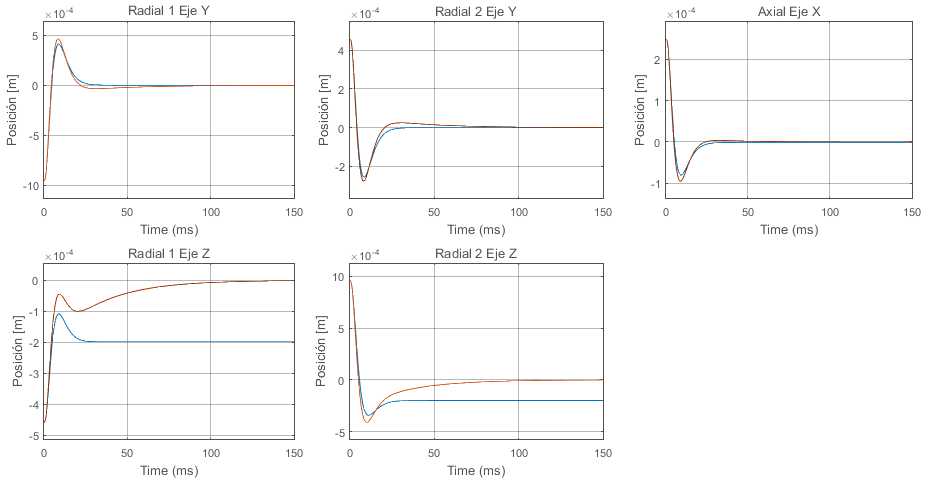
\includegraphics[width=\textwidth]{images/Capitulo_4_resultados_simulacion/simu_retroalimentado_vs_integral}
\caption{Salida del sistema. Control retroalimentado (azul) y Control integral(rojo).}
\label{fig:Controlador_retroalimentado_vs_Controlador_integral}
\end{center}
\end{figure}

La salida del sistema simulado mostrado en la figura \ref{fig:Controlador_retroalimentado_vs_Controlador_integral} representa el desplazamiento del eje medido desde los extremos del rotor. Podemos observar que ambos controladores llegan a estabilizar la posici�n del eje, sin embargo el sistema con controlador retroalimentado no converge en la posici�n deseada ($0$), en cambio el sistema con controlador integral s� lo hace.

\section{Controlador continuo y Controlador discreto} 

Esta simulaci�n consiste en un controlador integral continuo \ref{fig:esquema-controlador-integral} con observador de estados,  y sus versiones discretizadas \ref{fig:esquema-controlador-discreto} el cual opera con una frecuencia de muestreo de $10kHz$.

Esta simulaci�n se realiza sin cargas externas y con las condiciones iniciales:
\begin{equation}
	\begin{pmatrix}
	x_c \\ y_c \\ z_c \\ \dot{x}_c \\ \dot{y}_c \\ \dot{z}_c \\ \phi \\ \theta \\ \dot{\phi} \\ \dot{\theta}
	\end{pmatrix} = \begin{pmatrix}
	0.25mm \\ -0.25mm \\ 0.25mm \\ 0\frac{mm}{s} \\ 0\frac{mm}{s} \\ 0\frac{mm}{s} \\ -0.0015rad \\ 0.0015rad \\ 0\frac{rad}{s} \\ 0\frac{rad}{s}
	\end{pmatrix} 
\end{equation}

\begin{figure}[H]
\begin{center}
\centering
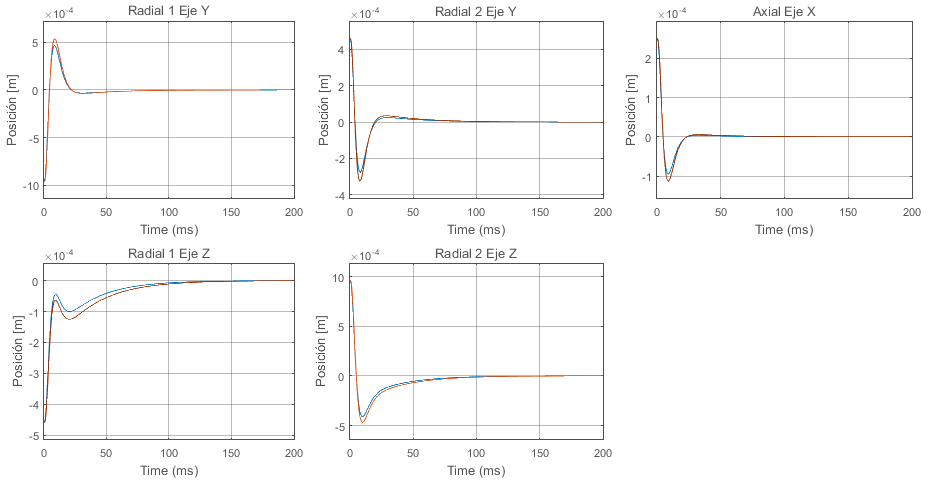
\includegraphics[width=\textwidth]{images/Capitulo_4_resultados_simulacion/simu_discreto_vs_continuo}
\caption{Salida del sistema. Control integral continuo (azul) y Control integral discreto(rojo).}
\label{fig:Controlador_continuo_vs_Controlador_discreto}
\end{center}
\end{figure}

En la figura \ref{fig:Controlador_continuo_vs_Controlador_discreto} podemos observar que ambos controladores se comportan de manera similar, validando que el controlador discreto emula correctamente al continuo.

\section{Controlador calendarizado}

Esta simulaci�n consiste en un controlador integral discreto \ref{fig:esquema-controlador-discreto} y en un controlador integral discreto calendarizado \ref{fig:esquema-controlador-calendarizado}, el controlador integral discreto fue linealizado en $\omega_s = 10000$. Estos operan con una frecuencia de muestreo de $10kHz$.

Esta simulaci�n se realiza sin cargas externas, con un $\omega_s = -30000$ y con las condiciones iniciales:

\begin{equation}
	\begin{pmatrix}
	x_c \\ y_c \\ z_c \\ \dot{x}_c \\ \dot{y}_c \\ \dot{z}_c \\ \phi \\ \theta \\ \dot{\phi} \\ \dot{\theta}
	\end{pmatrix} = \begin{pmatrix}
	0.25mm \\ -0.25mm \\ 0.25mm \\ 0\frac{mm}{s} \\ 0\frac{mm}{s} \\ 0\frac{mm}{s} \\ -0.0015rad \\ 0.0015rad \\ 0\frac{rad}{s} \\ 0\frac{rad}{s}
	\end{pmatrix} 
\end{equation}

\begin{figure}[H]
\begin{center}
\centering
\includegraphics[width=\textwidth]{images/Capitulo_4_resultados_simulacion/simu_normal_cal_mismo_ws}
\caption{Salida del sistema. Control integral discreto (azul) y Control integral discreto calendarizado (rojo)(ambas curvas superpuestas). $\omega_s = 10000$.}
\label{fig:Controlador_linealizado_vs_Controlador_calendarizado_ws_10000}
\end{center}
\end{figure}

Cuando la velocidad angular del rotor ($\omega_s$) es la misma que se us� durante el proceso de linealizaci�n, ambos controladores operan de la misma manera. Por lo tanto tienen respuesta iguales \ref{fig:Controlador_linealizado_vs_Controlador_calendarizado_ws_10000}.

\begin{figure}[H]
\begin{center}
\centering
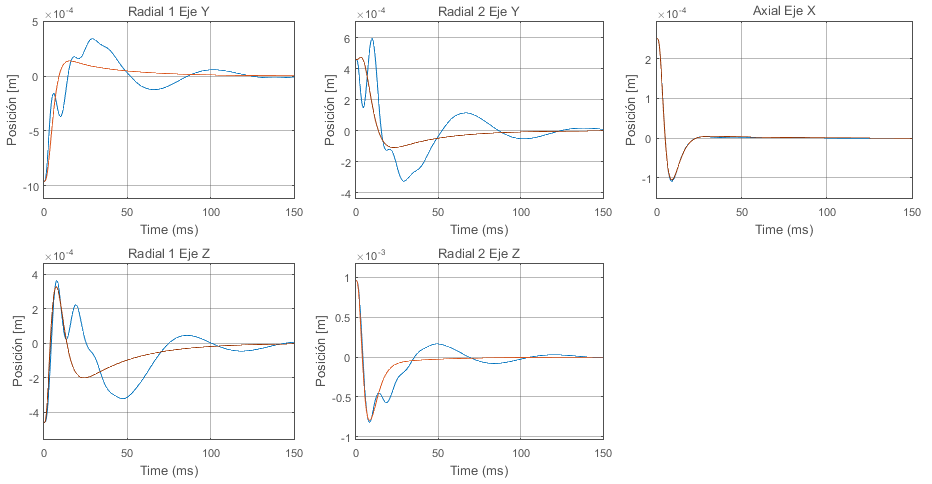
\includegraphics[width=\textwidth]{images/Capitulo_4_resultados_simulacion/normal_vs_calendarizado}
\caption{Salida del sistema. Control integral discreto (azul) y Control integral discreto calendarizado (rojo). $\omega_s = -30000$.}
\label{fig:Controlador_linealizado_vs_Controlador_calendarizado_ws_30000}
\end{center}
\end{figure}

Cuando trabajan a velocidades angulares diferentes, el controlador no calendarizado presenta problemas para estabilizar el rotor debido a los efectos de la precesi�n. En cambio el control calendarizado no presenta problemas.  

\section{Simulaci�n Accionamiento H�brido} 

Esta simulaci�n consiste en un controlador integral y observador discreto calendarizado con un $\omega_s = 10000$ y con las condiciones iniciales:

\begin{equation}
	\begin{pmatrix}
	x_c \\ y_c \\ z_c \\ \dot{x}_c \\ \dot{y}_c \\ \dot{z}_c \\ \phi \\ \theta \\ \dot{\phi} \\ \dot{\theta}
	\end{pmatrix} = \begin{pmatrix}
	0.1mm \\ -0.1mm \\ 0.1mm \\ 0\frac{mm}{s} \\ 0\frac{mm}{s} \\ 0\frac{mm}{s} \\ -0.001rad \\ 0.001rad \\ 0\frac{rad}{s} \\ 0\frac{rad}{s}
	\end{pmatrix} 
\end{equation}

y con una fuerza aplicada en el centro con valor de: 

\begin{equation}
	\begin{pmatrix}
	F_{dx} & F_{dy} & F_{dz}
	\end{pmatrix} = \begin{pmatrix}
		sen(100\pi)[N] & sen(200\pi)[N] & 3sen(200\pi) - 25 [N]
	\end{pmatrix}
\end{equation}

A diferencia de las simulaciones realizadas hasta ahora, la componente de fuerza $F_z$ del RMR es usada como se�al de control para el MCCE. A continuaci�n se simulan dos casos: (a) con el MCCE descativado y (b) con el MCCE activado.

\begin{figure}[H]
\begin{center}
\centering
\includegraphics[width=\textwidth]{images/Capitulo_4_resultados_simulacion/simu_mcce_respuesta_carga_combinada_desactivado}
\caption{Simulaci�n con carga combinada MCCE desactivado.}
\label{fig:Simulacion_carga_combinada_MCCE_desactivado}
\end{center}
\end{figure}

\begin{figure}[H]
\begin{center}
\centering
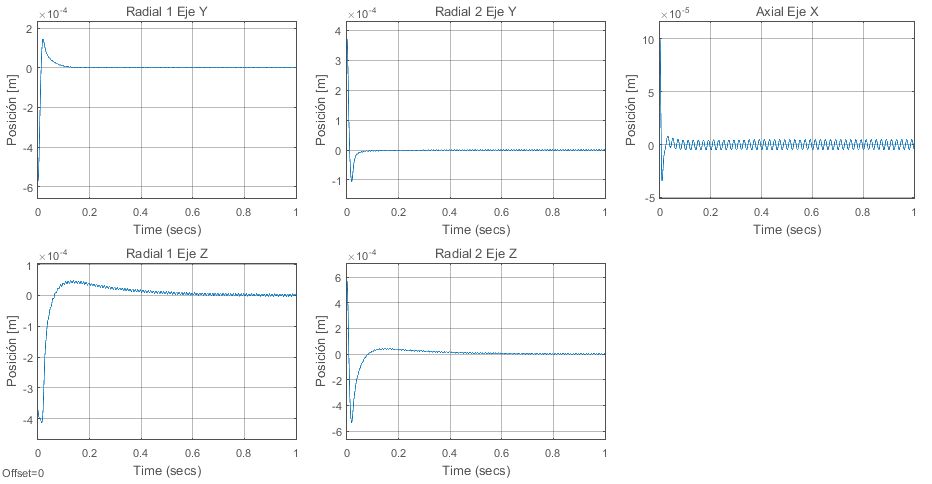
\includegraphics[width=\textwidth]{images/Capitulo_4_resultados_simulacion/simu_mcce_respuesta_carga_combinada}
\caption{Simulaci�n con carga combinada MCCE activado.}
\label{fig:Simulacion_carga_combinada_MCCE_activada}
\end{center}
\end{figure}

Se puede apreciar en la figura \ref{fig:Simulacion_carga_combinada_MCCE_desactivado} y \ref{fig:Simulacion_carga_combinada_MCCE_activada} que activar el lazo de control del MCCE no compromete la estabilidad del sistema. A continuaci�n se muestran los efectos en los electroimanes cuando se activa el MCCE. 

\begin{figure}[H]
\begin{center}
\centering
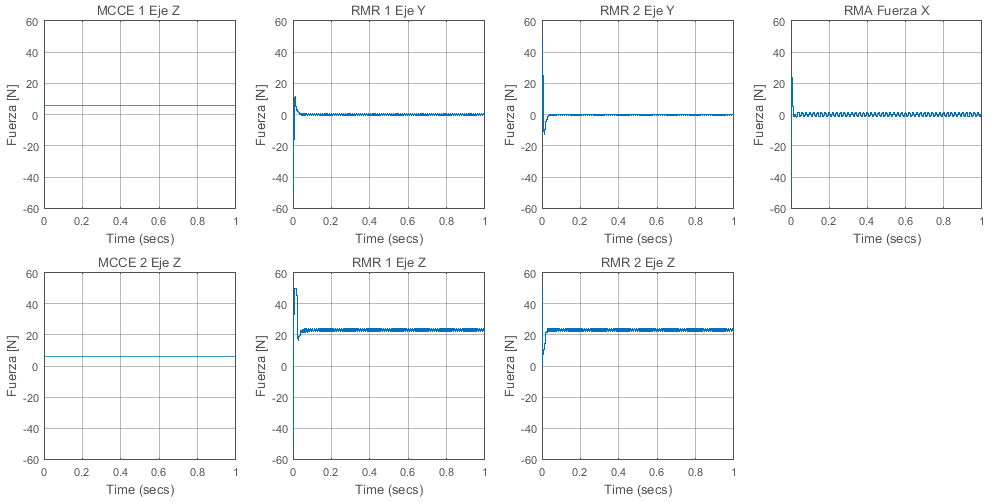
\includegraphics[width=\textwidth]{images/Capitulo_4_resultados_simulacion/simu_mcce_fuerzas_desactivado}
\caption{Fuerzas ejercidas por los electroimanes (MCCE desactivado).}
\label{fig:Simulacion_MCCE_desactivado}
\end{center}
\end{figure}

\begin{figure}[H]
\begin{center}
\centering
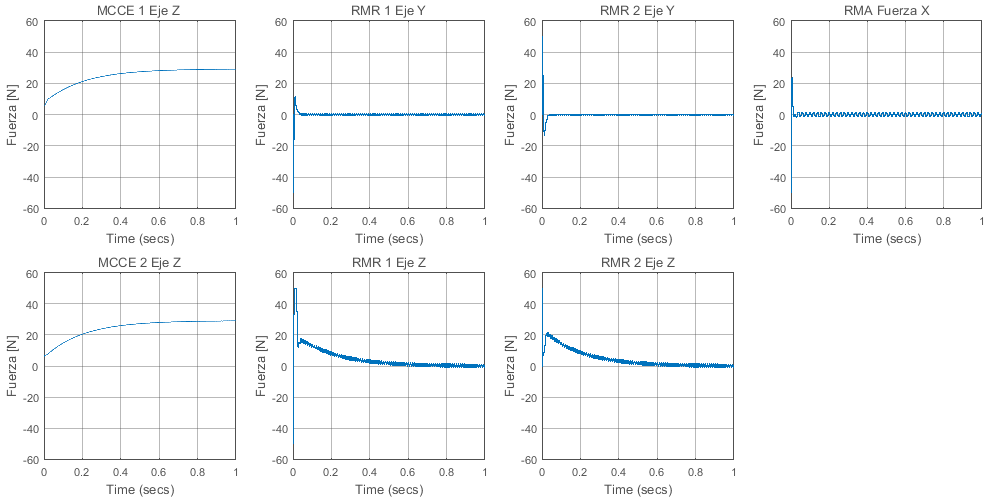
\includegraphics[width=\textwidth]{images/Capitulo_4_resultados_simulacion/simu_mcce_fuerzas_activo}
\caption{Fuerzas ejercidas por los electroimanes (MCCE activado).}
\label{fig:Simulacion_MCCE_activado}
\end{center}
\end{figure}

En el caso \textbf{(a)}, cuando el sistema se estabiliza, el MCCE mantiene una fuerza constante de $6 N$, mientras que el $RMR_z$ converge a una fuerza de $23 N$ (fig. \ref{fig:Simulacion_MCCE_desactivado}). En el caso \textbf{b}, la fuerza del MCCE converge a $29 N$, mientras que el $RMR_z$ converge a una fuerza aproximada de $0 N$.

En ambos casos, los controladores logran compensar las fuerzas combinadas que se les aplica y r�pidamente convergen al origen (fig. \ref{fig:Simulacion_carga_combinada_MCCE_desactivado}, \ref{fig:Simulacion_carga_combinada_MCCE_activada}).
